%% Submissions for peer-review must enable line-numbering
%% using the lineno option in the \documentclass command.
%%
%% Preprints and camera-ready submissions do not need
%% line numbers, and should have this option removed.
%%
%% Please note that the line numbering option requires
%% version 1.1 or newer of the wlpeerj.cls file.
\def\tightlist{}

\documentclass[fleqn,10pt,lineno]{wlpeerj} % for journal submissions
% \documentclass[fleqn,10pt]{wlpeerj} % for preprint submissions

\usepackage{longtable}
\usepackage{hyperref}
\PassOptionsToPackage{hyphens}{url}\usepackage{hyperref}
%\usepackage[hyphens]{url}

\title{The Effect of Tides on Nearshore Environmental DNA}

\author{Ryan P. Kelly}
\author{Ram\'{o}n Gallego}
\author{Emily Jacobs-Palmer}
\affil{University of Washington, School of Marine and Environmental Affairs, Seattle, Washington USA}
%\affil[1]%{Address of second author}
\corrauthor{Ryan P. Kelly}{rpkelly@uw.edu}

\begin{abstract}
Organisms of all kinds leave genetic traces in their environments, and in recent years, sequencing this environmental DNA (eDNA) has become a tractable means of surveying many species using water, air, or soil samples. The technique is beginning to become a core tool for ecologists, environmental scientists, and biologists of many kinds, but the temporal resolution of eDNA sampling is often unclear, limiting the ecological interpretations of the resulting datasets. Here, in a temporally and spatially replicated field study using ca. 330bp of eukaryotic COI mtDNA as a marker, we find that nearshore organismal communities are largely consistent across tides. Our findings suggest that nearshore eDNA tends to be endogenous to the site and water mass sampled, rather changing systematically as waters change over during the tidal cycle. However, where water-mass characteristics change, we find that the eDNA communities change in concert, again suggesting a close association between the habitat sampled and the eDNA community recovered. 
\end{abstract}

\begin{document}

\flushbottom
\maketitle
\thispagestyle{empty}

\section{Introduction}\label{introduction}

As environmental DNA (eDNA) becomes an increasingly important tool in
ecological research (Sigsgaard et al., 2016; Deiner et al., 2017), it is
critical to understand how techniques for eDNA collection and analysis
perform under real-world conditions (Port et al., 2016). In particular,
we must characterize the spatial and temporal resolution of
amplicon-sequencing studies in order to confidently identify ecological
patterns in the field (O'Donnell et al., 2017); like any sampling
technique, eDNA can reveal a phenomenon only where the effects of that
phenomenon are sufficiently large to be detected above background
variation (e.g., among replicates or time points).

Most efforts to quantify the behavior of eDNA in the field have taken
the form of quantitative PCR (qPCR) studies, in which the concentration
of a particular template DNA is measured over space or time. Notable
recent examples include documenting degradation of DNA over tens of
meters in the flow of artificial streams (Jerde et al., 2016), caging
trout and measuring eDNA concentration at intervals downstream (Jane et
al., 2015), estimating eDNA production and degradation over time in a
static environment (Sassoubre et al., 2016), and estimating production
and decay rates of eDNA from both caged and wild char in a field setting
(Wilcox et al., 2016), among others (e.g., Thomsen et al., 2012; Deiner
\& Altermatt, 2014). Although the precise findings vary by setting and
details of the molecular assay employed, even with highly sensitive
qPCR, the distance from its source that eDNA can reliably be detected
appears to be small, on the order of 10 -- 1000m.

By contrast, less work has focused on the behavior of eDNA as reflected
in ecological amplicon-sequencing studies. Port and colleagues showed
that vertebrate eDNA communities can be distinguished at intervals of
60m (Port et al., 2016) in nearshore marine waters, and O'Donnell et al.
(2017) suggested that a similar spatial scale (\textless{} 75m) pertains
to a broader nearshore metazoan dataset. These were each
single-time-point snapshots of animal species in dynamic environments,
however, and especially in marine and aquatic environments in which
spatial and temporal scales are linked by bulk transport of water, fine
spatial resolution could be obliterated by water movement.

Nearshore marine habitats are among the most physically dynamic and
biologically diverse on earth (Helmuth et al., 2006). The movement of
water associated with tide is a fundamental property of these
environments (Babson, Kawase \& MacCready, 2006), dramatically shaping
the life histories and ecology of organisms that live there.
Environmental DNA surveys hold particular promise for better
understanding thousands of species that may co-occur at a single
nearshore marine location. However, use of this technique in the
intertidal zone requires a practical knowledge of the effects of tide on
the presence of eDNA sequences. Moreover, the intertidal environment
provides rigorous testing grounds in which to discern the origins of
genetic material detected in eDNA surveys, more generally.

Given recent work suggesting that eDNA signals are predominantly highly
localized in space and time (Thomsen \& Willerslev, 2015, and references
therein) -- although in some circumstances, eDNA may travel some
distance (Deiner \& Altermatt, 2014) -- we asked whether marine eDNA
community composition changes over tidal cycles at a given location. A
scenario in which eDNA communities change in unpredictable ways with
each new tide would suggest an exogeneous origin for that DNA, such that
DNA arrives at a site with incoming tides, drawn from a pool of
organisms existing elsewhere. By contrast, consistent eDNA communities
over multiple tidal cycles would strongly suggest an endogenous origin
and highly localized signal.

Here, we find that nearshore COI eDNA community composition is not
strongly influenced by tide, and instead remains largely consistent
within each geographic location across multiple successive tides.
However, where shifts in the physical and chemical aqueous environment
occur, the eDNA community appears to change accordingly. It therefore
seems likely that changes in aqueous habitat characteristics -- not tide
itself -- yield changes in eukaryotic eDNA communities.

\section{Methods}\label{methods}

\subsection{Field Sampling}\label{field-sampling}

\begin{figure}[!ht]

{\centering 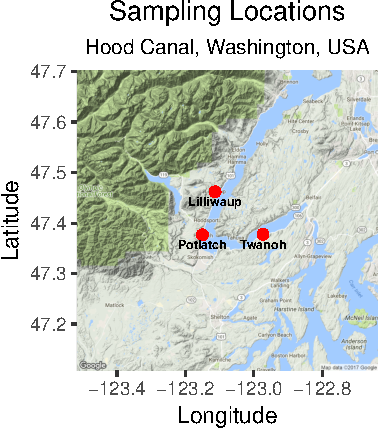
\includegraphics{figures/FIG1_sitemap-1} 

}

\caption{\label{fig:fig1}Nearshore sampling locations in Hood Canal, Washington, USA.}\label{fig:FIG1_sitemap}
\end{figure}

Our study design aimed to distinguish the effects of tide from
site-level community differences and from sampling error. Consequently,
we sampled each of three geographic locations (Fig 1; GPS coordinates
given in Suppl. Table 1) in Hood Canal, Washington, USA, four times --
twice during an incoming tide, and twice during an outgoing tide -- over
a ca. 28-hour period. Despite its name, the Hood Canal is in fact a
natural glacial fjord. We collected three 1-L water samples for eDNA
analysis (ca. 10m apart) at each site during each sampling event. No
permits were required for collecting water samples, given the inherently
public nature of saltwater in the United States. Each sample was
collected at the surface (\textless{} 1m depth), using a ca. 3m-long
pole with plastic collection bottle attached. We kept samples on ice
until they could be processed, which occurred within hours of
collection. We filtered 500mL from each sample onto cellulose acetate
filters (47mm diameter; 0.45um pore size) under vacuum pressure, and
preserved the filter at room temperature in Longmire's buffer following
Renshaw et al. (2015). Deionized water served as a negative control for
filtering. We measured water temperature and salinity with a hand-held
multiprobe (Hanna Instruments, Inc., model HI-9828), as well as
measuring salinity with a handheld manual refractometer; the latter
instrument more reliably reflected lab calibrations, and we use these
measurements here.

\begin{longtable}[]{@{}lcc@{}}
\caption{Samples by site and tide, showing balanced sampling design.
Each site (N = 3) had a total of 4 sampling events (time points),
consisting of 3 water samples per event, and then 3-4 PCR replicates per
water sample, such that we sequenced 36-44 individual PCR replicates per
geographic sampling site. 35 of 36 samples were successfully processed,
with 93 individual replicates survived quality-control, described
below.}\tabularnewline
\toprule
& Incoming Tide & Outgoing Tide\tabularnewline
\midrule
\endfirsthead
\toprule
& Incoming Tide & Outgoing Tide\tabularnewline
\midrule
\endhead
Lilliwaup & 5 & 6\tabularnewline
Potlatch & 6 & 6\tabularnewline
Twanoh & 6 & 6\tabularnewline
\bottomrule
\end{longtable}

\subsection{DNA Extraction, Amplification, and
Sequencing}\label{dna-extraction-amplification-and-sequencing}

We extracted total DNA from the filters using a
phenol:chloroform:isoamyl alcohol protocol following (Renshaw et al.,
2015), resuspended the eluate in 200uL water, and used 1uL of diluted
DNA extract (1:10) as template for PCR. Although a single locus cannot
completely characterize the biodiversity at a particular location (see,
e.g., Kelly et al., 2017), we used a 330bp fragment of COI to assess the
eukaryotic variance among our samples. This primer set (Leray et al.,
2013) amplifies a broad array of taxa including representative diatoms,
dinoflagellates, metazoans, fungi, and others; here, we simply use this
primer set as an assay to characterize community similarity among
samples. We followed a two-step PCR protocol to first amplify and then
index our samples for sequencing, such that we could sequence many
samples on the same sequencing run while avoiding amplification bias due
to index sequence (O'Donnell et al., 2016). PCR mixes were 1X HotStar
Buffer, 2.5mM \(MgCl_2\), 0.5mM dNTP, 0.3\(\mu\)M of each primer and
include 0.5 units of HotStar Taq (Qiagen Corp.) per 20 \(\mu\)L
reaction. The first round of PCR consisted of 40 cycles, including an
annealing touchdown from 62\(^\circ\)C to 46\(^\circ\)C (-1\(^\circ\)C
per cycle), followed by 25 cycles at 46\(^\circ\)C. The indexing PCR
used a similar protocol with only 10 cycles at 46\(^\circ\)C.

We generated three PCR replicates for each of 35 water samples (3
samples per sampling event, 4 sampling events per site, 3 sites = 36
water samples, of which 35 were processed successfully), and sequenced
each replicate individually in order to assess the variance in detected
eDNA communities due to stochasticity during amplification. We
simultaneously sequenced positive (Ostrich (\emph{Struthio camelus})
tissue, selected because of the absence of this species in our study
sites) controls with identical replication. We carried negative controls
through amplification, but did not sequence them, due to the practical
and theoretical issues associated with library preparation in samples
without any discernable amplicon. No amplification was visible via gel
elecrophoresis in the negative controls, and fluorometry (Qubit; Thermo
Scientific) analysis showed negligible amounts of DNA present in those
samples after amplification. The positive controls provided us with
consistent estimates of cross-contamination (see below), which we used
in sequence quality-control prior to analysis.

Following library preparation according to manufacturers' protocols
(KAPA Biosystems, Wilmington, MA, USA; NEXTflex DNA barcodes, BIOO
Scientific, Austin, TX, USA), sequencing was carried out on an Illumina
MiSeq (250bp, paired-end) platform in two different batches: a MiSeq V.2
run and a MiSeq nano run. These were processed separately through the
first stages of bioinformatics analysis (see below), and then combined
after primer removal for dereplication. PCR replicates (derived from the
same sampled bottle of water) sequenced on different runs clustered
together without exception (see Results), and thus combining the data
from two sequencing runs was appropriate.

\subsection{Bioinformatics}\label{bioinformatics}

We processed the resulting sequence reads with a custom Unix-based
script (O'Donnell, 2015), which calls third-party programs (Martin,
2011; Zhang et al., 2014; Mahé et al., 2015) to move from raw sequence
data to a quality-controlled dataset of counts of sequences from
operational taxonomic units (OTUs). A total of 5,105,198 reads survived
preliminary quality-control in the bioinformatics pipeline, representing
149,829 OTUs, most of which were rare (\textless{} 5 reads). We
controlled for contamination in three ways, following our approach in
(Kelly et al., 2017). First, to address the question of whether rare
OTUs are a function of low-level contamination or are true reflections
of less-common amplicons, we used a site-occupancy model to estimate the
probability of OTU occurrence (Royle \& Link, 2006; Lahoz-Monfort,
Guillera-Arroita \& Tingley, 2015), using multiple PCR replicates of
each environmental sample as independent draws from a common binomial
distribution. We eliminated from the dataset any OTU with
\textless{}80\% estimated probability of occurrence (a break point in
the observed distribution of occupancy probabilities), yielding a
dataset of 4,811,014 reads (7,503 OTUs). Second, we estimated (and then
minimized) the effect of potential cross-contamination among samples --
likely due to tag-jumping (Schnell, Bohmann \& Gilbert, 2015) or similar
effects -- as follows: (1) we calculated the maximum proportional
representation of each OTU across all control (here, ostrich) samples,
considering these to be estimates of the proportional contribution of
contamination to each OTU recovered from the field samples. (2) We then
subtracted this proportion from the respective OTU in the field samples,
yielding 4,370,486 reads (7,496 OTUs). Finally, we dropped samples that
had highly dissimilar PCR replicates (Bray-Curtis dissimilarities
\textgreater{} 0.49, which were outside of the 95\% confidence interval
given the best-fit model of the observed among-replicate
dissimilarities). The result was a dataset of 4,164,517 reads (7,496
OTUs), or 81.57\% of the post-pipeline reads. We rarefied read counts
from each PCR replicate to allow for comparison across water samples
using the vegan package for R (Oksanen et al., 2015), such that each
sample consisted of \(1.85 \times 10^4\) reads from 7,155 OTUs. We
carried out subsequent analyses on a single, illustrative rarefaction
draw; rarefaction draws did not vary substantially (Supplemental Figure
1).

All bioinformatics and other analytical code is included as part of this
manuscript, including OTU tables and full annotation data, and these
provide the details of parameter settings in the bioinformatics
pipeline. In addition, sequence data are deposited and publicly
available in GenBank (Upon Acceptance).

\subsection{Statistical Analysis}\label{statistical-analysis}

\subsubsection{Apportioning Variance in Bray-Curtis Dissimilarity Among
Sites, Sampling Events, Bottle Samples, and PCR
Replicates}\label{apportioning-variance-in-bray-curtis-dissimilarity-among-sites-sampling-events-bottle-samples-and-pcr-replicates}

We calculated the variance in OTU communities at five hierarchical
levels -- between tides (incoming vs.~outgoing), among geographic sites
(N = 3), among sampling events within geographic sites (N = 4 per site),
among sample bottles within a sampling event (N = 3 per event per site),
and among PCR replicates (N = 3 per individual sample bottle; reflected
by the model residuals) -- using a PERMANOVA test on Bray-Curtis (OTU
count data) dissimilarity among sequenced replicates. Calculations were
carried out in R ver. 3.3.1 (R Core Team, 2016) using the vegan (Oksanen
et al., 2015) package. Having established that the variance among PCR
replicates and bottles was small relative to variance among sampling
events and geographic sites (see Results), it was clear that our dataset
had the necessary resolution to detect community-level changes -- if any
-- associated with changes in tide.

\subsubsection{How Many Ecological Communities Are
Present?}\label{how-many-ecological-communities-are-present}

We then used Bray-Curtis dissimilarity to visualize differences among
sampled communities at each hierarchical level of organization, using
ordination (NMDS, Venables \& Ripley, 2002), treemaps (Wickham, 2009;
Wilkins), and a heatmap. Given the strong and consistent differentiation
we identified between two ecological communities in the eDNA data (see
Results), we then labeled these communities 1 and 2, and applied a set
of standard statistics to test for associations between community
identity and geographic site (Fisher's exact test), tidal direction
(incoming vs.~outgoing; \(\chi^2\)), and tidal height (logistic
regression).

\subsubsection{Community Identity by Site and
Tide}\label{community-identity-by-site-and-tide}

We recovered tidal height data for our study sites during the relevant
dates from the National Oceanographic and Atmospheric Administration
data for Union, Washington (available at: \url{https://}
tidesandcurrents.noaa.gov/ noaatidepredictions.html).

\subsubsection{Characterizing the Observed Ecological
Communities}\label{characterizing-the-observed-ecological-communities}

A single genetic locus provides only a biased and incomplete view of an
ecosystem (see Kelly et al. (2017) for discussion), and although our
purpose was to test for the effect of tidal fluctuations on detected
eDNA communities -- which does not require taxonomic annotation of the
recovered OTUs -- we were nevertheless interested in the membership of
the ecological communities we detected. Our locus of choice, COI,
provided a broad view of ecosystem with 23 phyla in 8 kingdoms
represented (see Supplemental Table 2 for summary table). Algae
dominated the read counts, with approximately 91\% of annotated reads
mapped to taxa in the groups Chlorophyta and Phaeophyceae.

We assigned taxonomy to each OTU sequence using blastn (Camacho et al.,
2009) on a local version of the full NCBI nucleotide database (current
as of August 2017), recovering up to 100 hits per query sequence with at
least 80\% similarity and maximum e-values of \(10^{-25}\) (culling
limit = 5), and reconciling conflicts among matches using the last
common ancestor approach implemented in MEGAN 6.4 (Huson et al., 2016).
93.08\% of rarefied OTUs could be annotated at some taxonomic level,
with over half (57.54\%) being annotated to the level of taxonomic
Family or lower.

We report an index of community-wide changes across sampling events
using the top 10 most-common taxonomic Families in the dataset. We
carried out a finer-grained analysis to identify the OTUs driving the
observed community shifts at Twanoh by first using a cannonical
correspondence analysis (CCA; Oksanen et al., 2015), constrained by
community identity (1 vs.~2, identified via NMDS; see Results), then
filtering the CCA scores by read count, such that we plotted only OTUs
that strongly differentiated communities and that occurred at least 1000
times in the dataset. We then show these by Family-level taxonomic
annotation.

\section{Results}\label{results}

\subsection{Community-Level similarity among replicates, sites, etc:
Apportioning variance in Bray-Curtis
Dissimilarity}\label{community-level-similarity-among-replicates-sites-etc-apportioning-variance-in-bray-curtis-dissimilarity}

To evaluate the spatial and temporal turnover between eDNA communities,
we first apportioned the observed variation in COI Bray-Curtis
dissimilarities (calculated using OTU read counts) among tides (incoming
vs.~outgoing), sampling sites, sampling events within a site, biological
replicates (individual bottles of water taken during the same sampling
event), and technical replicates (PCR replicates from the same bottle of
water). Across the whole dataset, ecological communities at different
sampling sites (20-50km apart) account for the largest fraction of the
variance (0.43; Figure 2), and different sampling events within those
sites account for the next highest proportion (0.31). In contrast,
biological replicates (N = 3 bottles of water per sampling event, taken
ca. 10m apart) account for a small fraction (0.07) of the variance, with
differences among tides accounting for the smallest fraction of the
variance in community dissimilarity (0.06). The remainder -- 0.13 -- is
largely due to differences among technical PCR replicates (N = 3 per
bottle of water), much of which derives from stochasticity in the
presence of rare OTUs (Supplemental Figure 1). The comparitively low
variance issuing from biological and technical replicates relative to
sampling events and sites affords the resolution necessary to further
examine questions of community composition across space and time.

\begin{figure}[!ht]

{\centering 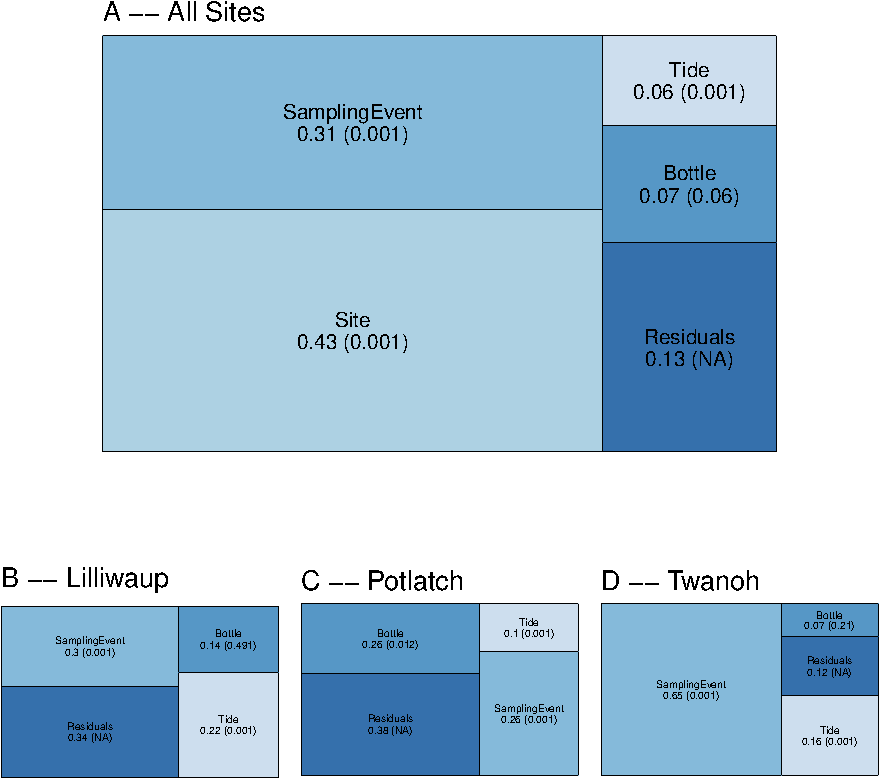
\includegraphics{figures/FIG2_ADONIS_TreemapDiagrams-1} 

}

\caption{\label{fig:AdonisFigure}Results of PERMANOVA, apportioning variance by hierarchical levels of sampling design: Tide (incoming vs. outgoing), Sampling Site, Sampling Event (N = 4 time points per site), and Sampling Bottle (N = 3 bottles per sampling event). Residuals reflect variance among PCR replicates (N = 3 replicates per sampling bottle) as well as variation due to rarefaction stochasticity and other sampling effects. The upper panel reflects results for the dataset as a whole, with lower panels giving site-specific variances. Numbers reflect proportion of the variance explained by the indicated hierarchical level (R$^2$), with permutation-derived p-values in parentheses.}\label{fig:FIG2_ADONIS_TreemapDiagrams}
\end{figure}

To examine the effect of tide at each of our three geographic locations
independently, we again apportioned variance among sampling event, tide,
sampling bottles (biological replicates), and PCR replicate (residuals;
Figure 2). Analyzing individual site-level data in this way eliminates
the portion of variance due to between-site differences, effectively
amplifying the contributions of the remaining hierarchical sampling
levels, including tide. Because we treat tidal direction (incoming
vs.~outgoing) as the highest hierarchical level, we are effectively
asking whether eDNA assays reflect a coherent ``incoming'' tidal
community and a coherent ``outoging'' tidal community across all sites.
For each of our three sampling locations, variation among sampling
events remains greater than variation between incoming and outgoing
tides (Figure 2b), with little evidence of consistent incoming or
outgoing tidal communities.

\begin{figure}[!ht]

{\centering 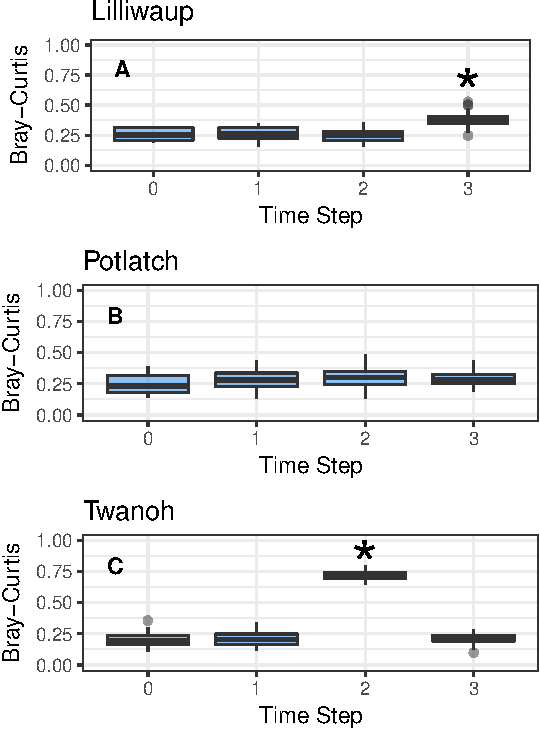
\includegraphics{figures/FIG3_BrayCurtis_timeSeries-1} 

}

\caption{\label{fig:TimeSeriesFigure}Comparison of Bray-Curtis dissimilarities within a reference sampling event (Time step = 0) and between the reference sample and subsequent samples at the same site (Time Steps 1, 2, and 3). Subsequent time steps reflect the accumulation of ecological eDNA differences over hours as the tide moves in and out. Sites shown individually. Steps with significant increases (Kruskal; p $<$ 0.01) marked with asterisks and discussed in the text. Y-axes identical to facilitate comparison across sites.}\label{fig:FIG3_BrayCurtis_timeSeries}
\end{figure}

We next tested the possibility that eDNA sequences might still regularly
shift in association with tide, even if not between two predicable
assemblages (see above). Conceiving of tidal turnovers within a site as
a series of events that could each influence community composition, we
treated our first sampling event at a site as the reference point for
that site, and assessed the Bray-Curtis dissimilarity of eDNA sequences
with each subsequent sampling event occurring at a later point in time
and after one or more changes in tide (Figure 3). If ecological
communities within each site remain consistent over time, we expect the
Bray-Curtis values of the community at time zero (the reference
community) vs.~time one (the subsequent sampling event) to be identical
to the dissimilarity values among bottles taken within the same sampling
event. We observe little change in community dissimilarity as a function
of tidal change (or indeed of time).

In all three sites, Bray-Curtis values remain stable across multiple
tide changes, with no continuously increasing trend over time. Instead,
two events stand out as statistically significant (Kruskal-Wallis, p
\textless{} 0.01): a moderate increase at Lilliwaup at time step 3 (ca.
26 hours after the reference sample, from median 0.26 to 1), and a far
larger jump in a single time point at Twanoh (ca. 19 hours after
reference; from 0.2 to 0.72, before returning to its reference value in
the subsequent sampling event). In each of these events, a change in
salinity of the sampled water is significantly associated with the
change in ecological community, while time-since-reference is not
(linear models; Lilliwaup t-value Salinity = 3.96 and
Time-since-reference = 0.65; Twanoh t-value Salinity = 3.63 and
Time-since-reference = 0.17; note that time-since-reference necessarily
encompasses tidal changes in our sampling scheme; See Supplemental
Figure 3 for site-level regressions with between Bray-Curtis
dissimilarities and changes in salinity).

In sum, neither tidal direction (incoming vs.~outgoing) nor individual
tidal events therefore consistently drive differences in sampled eDNA
communities, but as described below, individual environmental changes in
such as those seen in the Twanoh changeover event bear further scrutiny.

\subsection{How Many Ecological Communities Are
Present?}\label{how-many-ecological-communities-are-present-1}

\begin{figure}[!ht]

{\centering 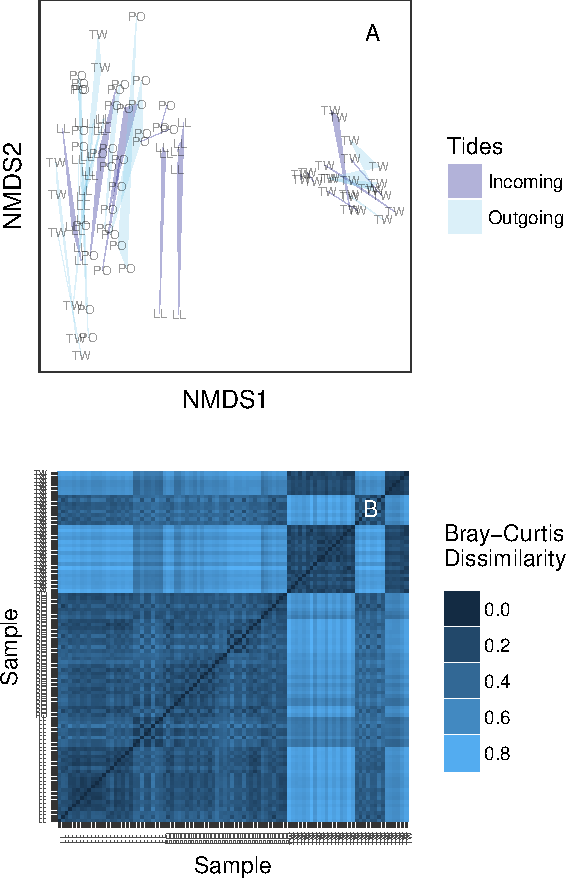
\includegraphics{figures/FIG4_multiplot_NMDS_BottleTide-1} 

}

\caption{\label{fig:fig4}(A) Ordination plot (non-metric multidimensional scaling; NMDS) plot of Bray-Curtis dissimilarities among sequenced replicates, by sampling bottle (polygon) and tide (polygon color). Polygons connect communities sequenced from replicate PCR reactions of the same sampled bottle of water. (B) The same data shown as a heatmap, ordered by site identity. Only the Twanoh samples (upper right) stand out as having substantial heterogeneity, reflecting the two different communities present during different sampling events at that site. Site labels: TW = Twanoh, PO = Potlatch, LL = Lilliwaup.}\label{fig:FIG4_multiplot_NMDS_BottleTide}
\end{figure}

We created an ordination plot of Bray-Curtis distances among each of our
sequenced replicates to visualize any distinct ecological communities
present in the dataset (Figure 4a). In agreement with the analysis of
variance, technical PCR replicates and biological replicates
consistently cluster closely in ordination space, yet two
non-overlapping eDNA sequence assemblages appear on this plot. A heatmap
of the same Bray-Curtis values reveals the underlying magnitudes of
dissimilarity and clustering, showing two clearly distinct communities
of eDNA sequences (Fig 4b). The two observed clusters are primarily
associated with sampling site: the left-hand community (ordination plot;
Fig 4a) is present in all technical and environmental replicates of all
Lilliwaup and Potlatch samples, and in all such replicates from a single
Twanoh sampling event. We call this ``community 1'' below. By contrast,
the right-hand community (``community 2'') is only present in the
remaining three Twanoh samples.

\subsection{Community Identity by Site and
Tide}\label{community-identity-by-site-and-tide-1}

\begin{figure}[!ht]

{\centering 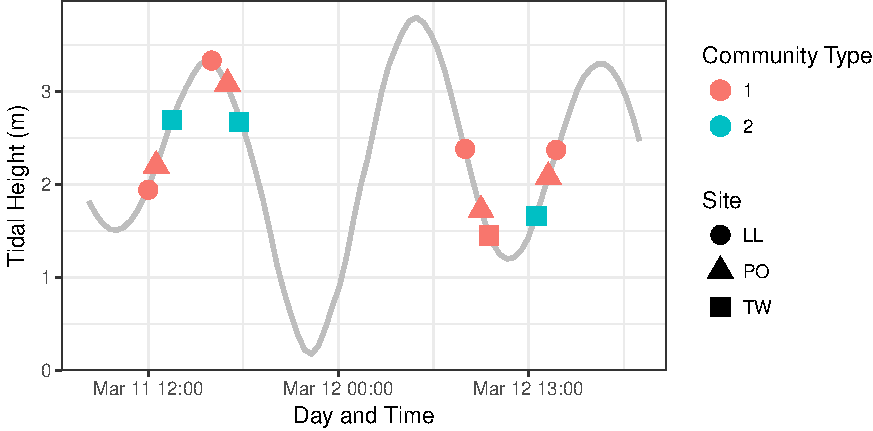
\includegraphics{figures/FIG5_tide_community_figure-1} 

}

\caption{\label{fig:fig5}eDNA Communities by Time, Tide, and Site. We identify community type 1 as the dominant eDNA community (as seen in Figure 4, which appears at every geographic site), and community type 2 as the distinct type occurring only at Twanoh. See text for community descriptions.}\label{fig:FIG5_tide_community_figure}
\end{figure}

To further investigate the relationship of each eDNA community with
tide, we first assigned membership of each sample to one of the two
communities based on a visual examination of our ordination analysis
(Figure 4a; polygon color) and plotted community membership of each
sample across the tidal cycle during collection (Figure 5). Both figures
qualitatively indicate a lack of association between tidal direction or
height and either of the two eDNA communities. Quantitatively, by
sampling event, community is independent of tidal height (p = 0.39;
linear regression) and of tidal direction (incoming vs.~outgoing; p =
0.163; \(\chi^2\)), but is related imperfectly to site identity (p =
1.554e-15; Fisher's exact test). The fact that Twanoh hosts different
communities at different times indicates that geography does not fully
explain differences between these communities, and that ecological
variables warrant further investigation as driving differences in
communities.

\subsection{Environmental Co-variates Assocated with Community
Change}\label{environmental-co-variates-assocated-with-community-change}

To identify ecological factors that might distinguish the two eDNA
assemblages observed, we modeled the association of each sample's
temperature, salinity, and site identity with communities 1 and 2.
Salinity and temperature explain nearly all of the variance in community
type (logistic regression best-fit model; null deviance = 84.79,
residual deviance = 1.033e-09): we observe community 2 in fresher
(\textless{} 20ppt salinity) and colder (\textless{} 9\(^\circ\)C) water
than we find community 1. Twanoh, in the southeastern portion of Hood
Canal most distant from the ocean, routinely experiences these kinds of
fresher, colder water events in our sampling month (March), unlike the
main stem of the Canal (Supplemental Figure 4).

In summary, the eDNA communities are more closely associated with
ecological variables -- salinity and temperature -- than with tide, or
even with geographical origin. This suggests that the two eDNA
assemblages may represent different aqueous habitat types, and led us to
investigate their taxonomic composition. We summarize the ecological and
biological context of each community sample in Figure 6, before
highlighting the taxa that are particularly influential in defining the
two communities.

\subsection{Taxa Associated with Distinct
Communities}\label{taxa-associated-with-distinct-communities}

\begin{figure}[!ht]

{\centering 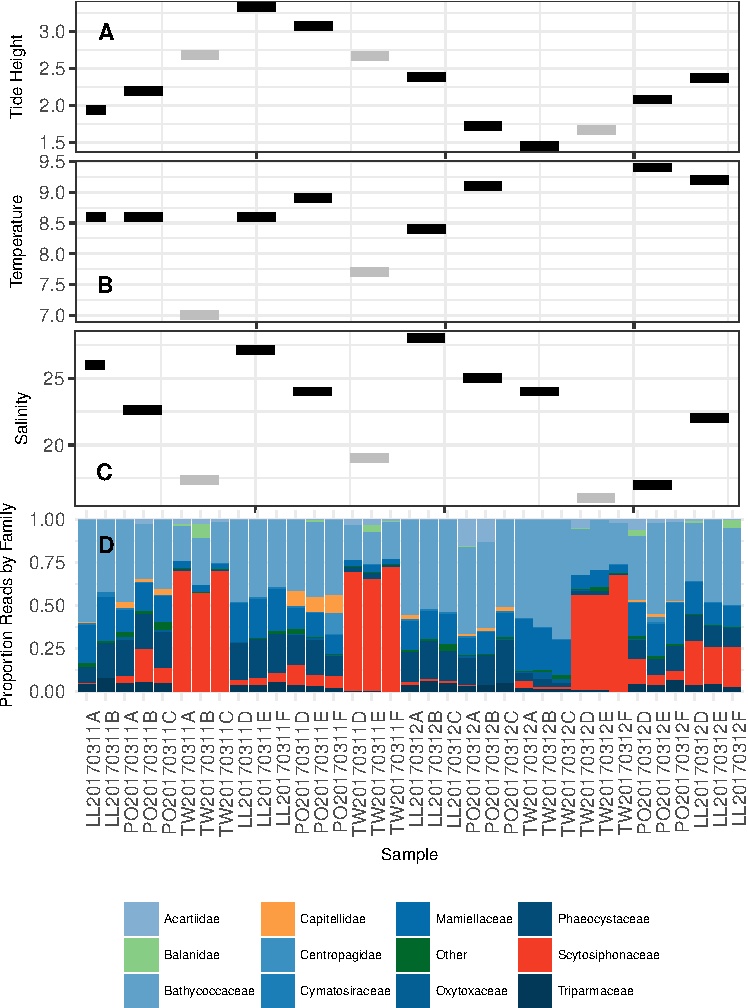
\includegraphics{figures/FIG6_multiplot_community_membership-1} 

}

\caption{\label{fig:fig6}Tidal height (m), Water temperature (C), Salinity (ppt), and proportion of DNA reads allocated among the top 10 Families in the annotated dataset. Two temperature points are missing due to a failure of equipment.}\label{fig:FIG6_multiplot_community_membership}
\end{figure}

To identify the taxonomic groups that most strongly differentiate
ecological communities 1 and 2 at Twanoh, the location at which we
detected both communities at different points in time, we performed a
constrained canonical correspondence analysis (CCA) principal component
analysis on the OTU counts. We constrained the ordination by community
identity as determined by the distance analyses above and filtered for
highly discriminating OTUs with high read counts (\textgreater{} 1000
reads) to identify a set of high-leverage taxa distinguishing
communities. The result was seven Families (Fig 7), two of which are
animals -- Balanidae (barnacles; sessile as adults) and Acartiidae
(copepods; planktonic) -- and the others of which are autotrophic groups
consisting of dinoflagellates (Oxytoxaceae), chlorophytes (Mamiellaceae,
Bathycoccaceae), a sessile brown alga (Scytosiphonaceae), and a another
heterokont, Triparmaceae. A handful of taxa therefore distinguishes the
two communities we identify with COI. However, given the well-known
effects of primer bias -- by which the apparent abundance of some taxa
can be grossly distorted by equating read count to organismal abundance
-- we stress that here we are using a single primer set as an index of
community similarity, rather than as an accurate reflection of the
abundances of taxa present in the water.

\begin{figure}[!ht]

{\centering 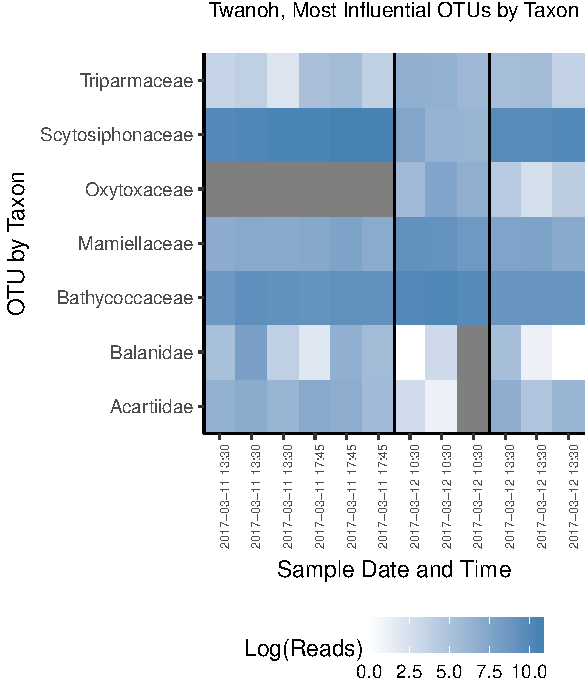
\includegraphics{figures/FIG7_TW_Families_turnover-1} 

}

\caption{\label{fig:fig7}Most influential OTUs, plotted by taxonomic Order, distinguishing the two ecological communities observed in water samples from Twanoh State Park. Shown are the taxonomic Families of OTUs with at least 1000 reads in the rarefied dataset, and having a constrained canonical correspondence analysis (CCA) score of greater than 0.7 (absolute value), which in our dataset most clearly divides the two communities. See text for CCA details. The vertical black lines in the chart delineate the communities identified previously by NMDS (see Figure 3a), with the time of each sample given along the x-axis, showing the shift from one community to the other -- and then largely back again -- within less than 24 hours. Note that each block of samples reflects a different point in the tidal cycle, and that the first two time points indicate a continuity of community membership despite a change in tide (see Figure 4).}\label{fig:FIG7_TW_Families_turnover}
\end{figure}

\section{Discussion}\label{discussion}

Environmental DNA is rapidly becoming an essential and widely-used tool
to identify community membership in aquatic environments (Taberlet et
al., 2012; Spear et al., 2015; Thomsen \& Willerslev, 2015; Kelly et
al., 2016; Yamamoto et al., 2016; Deiner et al., 2017). It is not yet
clear to what extent the sequences identified in eDNA studies reflect
the presence of local organisms in time and space, however (Jane et al.,
2015; Port et al., 2016; Wilcox et al., 2016). Of particular interest in
marine systems is the influence of tide on the detection of ecological
communities: must sampling schemes standardize tidal height and
direction during collection to detect consistent groups of species? Does
each tide bring with it a turnover in water, carrying exogenous DNA, or
do the sequences detected at any given time accurately reflect the
species present within a habitat in that moment? But more generally for
eDNA studies, to what extent must we worry about where DNA comes from
and where it goes? To address these questions, we collected and analyzed
eDNA communities at three different sites along the Hood Canal over the
course of multiple tidal turnovers. Thus, for each site, we were able to
examine the influence of reversals in tidal direction and larger-scale
changes in the water present at our study sites.

When analyzed together, eDNA collections from three locations
(Lilliwaup, Potlatch, and Twanoh) show substantial variance in OTU
membership and prevalence associated primarily with geographic location
(Figure 2). Grouping of samples in ordination space is also strongly
associated with site, rather than with tide (Figure 4a). Together, these
results suggest that eDNA surveys designed to clarify relationships
between distinct ecological communities are not likely to suffer
substantially from sample collection at varying points in the tidal
cycle, because the twice-daily exchange of water into- and out of our
sampling sites appeared to have little influence on the sequences
detected overall.

Although the effect of tide on eDNA community composition is small when
multiple geographic sites are considered simultaneously, tidal direction
may still influence the OTUs detected within a single location. The
existence of among-site differences in ecological communities in fact
provide the resolution necessary to detect such a local influence of
tide, if present - exogenous DNA arriving periodically with tidal flow
at each site might closely resemble neighboring communities, and differ
consistently from endogenous DNA collected on the ebb tide, which has
spent hours in contact with local benthic flora and fauna. A
site-by-site analysis reveals that a significant proportion of the
variance in OTU counts is associated with tide, but never as much as is
associated with differences between sampling events (Figure 2). These
results suggest community variance among individual sampling events,
although small in an absolute sense, dominates changes at the site scale
and accordingly that there is no coherent incoming- or outgoing-tide
eDNA fauna. Additionally, the eDNA community present at a single site
tends to drift little over time and with successive tidal turnovers
(Figure 3), instead changing in association with changes in salinity and
temperature of the water mass present at the time of sampling (Figure 6,
Supplemental Figure 3). Together, these results suggest that the effect
of tidal flow, \emph{per se}, on eDNA community membership is minimal
relative to the differences associated with changes in water
characteristics and geographic site.

Rather than tide, ecological variables such as temperature and salinity,
each of which differ among sites and sampling events, drive the bulk of
the variance in eDNA community membership (Figure 6 and multiple
regression). At Twanoh, we sampled by chance a dramatic shift in species
composition from community 2 to community 1 within the span of just a
few hours, and a concomitant shift towards warmer, more saline water
relative to baseline. Of the seven families most notably associated with
this turnover, four single-celled planktonic taxa (Triparmaceae,
Oxytoxaceae, Mamiellaceae, and Bathycoccoceae) increased in OTU count
with intrusion of the warmer, saltier water mass. By contrast, two
families with sessile adults (Balanidae and Scytosiphonaceae) and one
planktonic animal (Arctiideae) decreased (Figure 7). These results
broadly suggest that eDNA survey methodology succeeds in identifying the
planktonic species physically present within the water column at the
time of sampling. Additionally, the entrance and exit of a mobile,
aqueous habitat with characteristics more common at neighboring sites
diminishes but does not eradicate the signal from sessile groups. In
summary, the sequenced eDNA community reflects contributions from both
organisms living within the water itself, as well as immobile species in
contact with that more mobile community.

Taken together, our results suggest that eDNA samples taken from even
highly dynamic environments reflect recent contributions from local
species. With the exception of the occasional movement of water masses
representing distinct habitats for planktonic organisms, the eDNA
communities we sampled at three geographic sites were largely stable
over time and tide. Practically, this suggests that intertidal eDNA
research should be performed with substantial attention to ecological
variables such as temperature and salinity, which serve as markers of
the aqueous habitat present and which may not remain consistent
geographically. In contrast, tidal turnover itself appears to be a
secondary consideration that does not dramatically or consistently
affect the commmunity sampled, even within a single geographic location.
Marine intertidal eDNA surveys therefore appear to reflect the
endogenous DNA of the organisms present in the water and on the benthic
substrate at the time of sampling.

\subsection{Acknowledgements}\label{acknowledgements}

We thank K. Cribari for lab assistance, as well as R. Morris, G. Rocap,
and V. Armbrust at the UW Center for Environmental Genomics. Special
thanks to M. Kelly, A. Ramón-Laca, and E. Flynn for facilitating
fieldwork, and Julieta, Damián, and Owen for field assistance. We are
also greatful to L. Park, J. O'Donnell, K. Nichols, and P. Schwenke at
NMFS for sequencing support and expertise.

\subsection{Funding}\label{funding}

This work was made possible by grant 2016-65101 from the David and
Lucile Packard Foundation to RPK. The funders had no role in study
design, data collection and analysis, decision to publish, or
preparation of the manuscript.

\subsection{Grant Disclosures}\label{grant-disclosures}

The following grant was disclosed by the authors: David and Lucile
Packard Foundation: 2016-65101.

\newpage

\section{Supplemental Information}\label{supplemental-information}

\begin{table}

\caption{\label{tab:Supplement_GPScoordinatesSamplingAreas}Supplemental Table 1: Sampling Sites in Hood Canal, Washington, USA. Samples were taken intertidally, in water less than 1m deep.}
\centering
\begin{tabular}[t]{c|c|c}
\hline
Site & Latitude & Longitide\\
\hline
Lilliwaup State Park & 47.46 & -123.1\\
\hline
Potlatch State Park & 47.38 & -123.2\\
\hline
Twanoh State Park & 47.38 & -123.0\\
\hline
\end{tabular}
\end{table}

\begin{longtable}[]{@{}cccccc@{}}
\caption{Summary of unique annotations, by taxonomic rank, in the COI
dataset.}\tabularnewline
\toprule
Kingdom & Phylum & Classes & Orders & Families &
OtherRank\tabularnewline
\midrule
\endfirsthead
\toprule
Kingdom & Phylum & Classes & Orders & Families &
OtherRank\tabularnewline
\midrule
\endhead
Bacteria & Proteobacteria & 4 & 4 & 2 & 0\tabularnewline
Diatoms & Bacillariophyta & 11 & 17 & 24 & 5\tabularnewline
Dinoflagellates & Dinoflagellata & 7 & 12 & 12 & 0\tabularnewline
Fungi & Ascomycota & 5 & 7 & 10 & 6\tabularnewline
Fungi & Basidiomycota & 2 & 3 & 3 & 2\tabularnewline
Fungi & Mucoromycota & 1 & 1 & 1 & 0\tabularnewline
Heterokonta & Phaeophyceae & 6 & 14 & 37 & 4\tabularnewline
Metazoa & Annelida & 5 & 9 & 12 & 4\tabularnewline
Metazoa & Arthropoda & 20 & 67 & 80 & 43\tabularnewline
Metazoa & Brachiopoda & 0 & 0 & 1 & 0\tabularnewline
Metazoa & Bryozoa & 1 & 1 & 1 & 0\tabularnewline
Metazoa & Chordata & 13 & 16 & 17 & 3\tabularnewline
Metazoa & Cnidaria & 5 & 13 & 18 & 4\tabularnewline
Metazoa & Echinodermata & 1 & 1 & 2 & 0\tabularnewline
Metazoa & Gastrotricha & 1 & 1 & 1 & 0\tabularnewline
Metazoa & Mollusca & 7 & 20 & 23 & 3\tabularnewline
Metazoa & Nematoda & 1 & 1 & 1 & 0\tabularnewline
Metazoa & Nemertea & 1 & 2 & 2 & 2\tabularnewline
Metazoa & Porifera & 7 & 7 & 7 & 1\tabularnewline
Metazoa & Rotifera & 1 & 1 & 1 & 1\tabularnewline
Rhodophyta & Rhodophyta & 5 & 13 & 15 & 0\tabularnewline
Viridiplantae & Chlorophyta & 5 & 7 & 11 & 3\tabularnewline
Viridiplantae & Streptophyta & 4 & 4 & 4 & 0\tabularnewline
\bottomrule
\end{longtable}

\begin{figure}[!ht]

{\centering 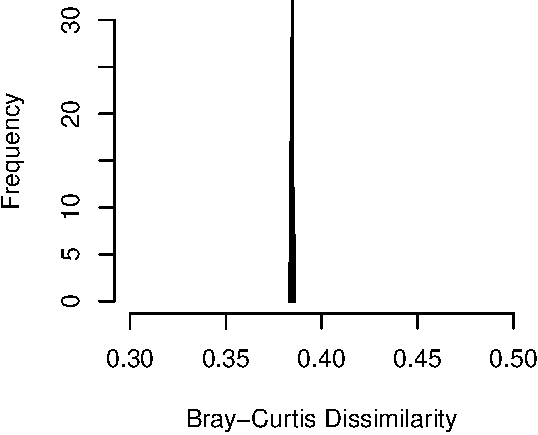
\includegraphics{figures/Supplement_Rarefaction_data-1} 

}

\caption{\label{fig:SuppFig1} Differences among rarefaction draws expressed as median Bray-Curtis dissimilarities. The lack of variation in median dissimilarity among rarefaction draws underscores the fact that the results we present in the main manuscript do not differ substantially among different rarefaction draws.}\label{fig:Supplement_Rarefaction_data}
\end{figure}

\begin{figure}[!ht]

{\centering 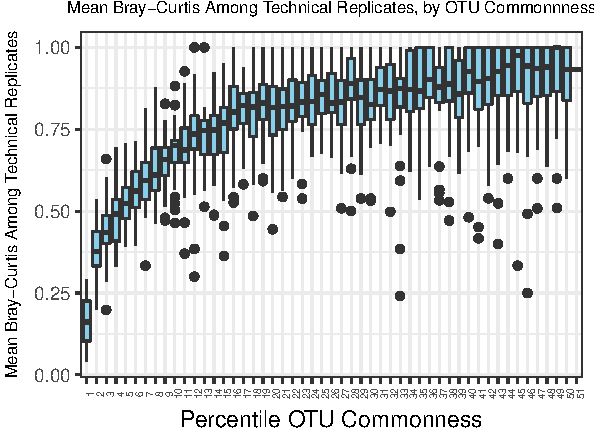
\includegraphics{20171117_Tides_and_eDNA_RPK_files/figure-latex/stochastic_variation_rareTail-1} 

}

\caption{\label{fig:SuppFig2}Variation among technical (PCR) replicates, expressed as Bray-Curtis dissimilarity among replicates using data subsets according to OTU commonness. Replicates are similar with respect to common OTUs, but stochasticity quickly dominates as OTUs become rarer, such that PCR replicates appear quite different with respect to OTUs in the bottom 90 percent of commonness.}\label{fig:stochastic_variation_rareTail}
\end{figure}

\begin{figure}[!ht]

{\centering 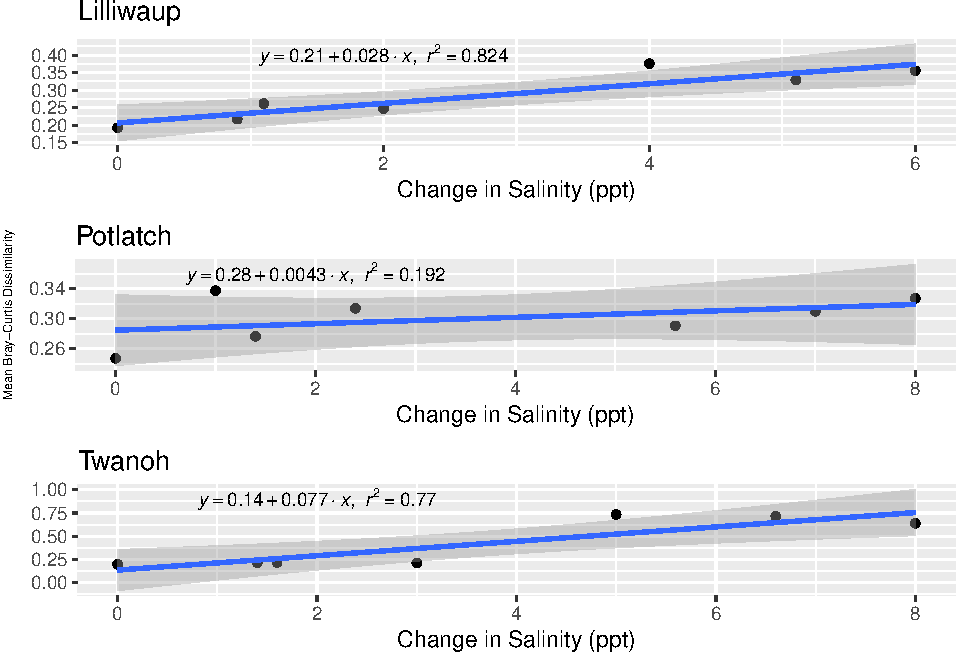
\includegraphics{20171117_Tides_and_eDNA_RPK_files/figure-latex/salinity_BC_correlations-1} 

}

\caption{\label{fig:SupplFig3}Changes in eDNA community are associated with changes in salinity at each site; note the different scales in both the x and y axes.}\label{fig:salinity_BC_correlations}
\end{figure}

\begin{figure}[!ht]

{\centering 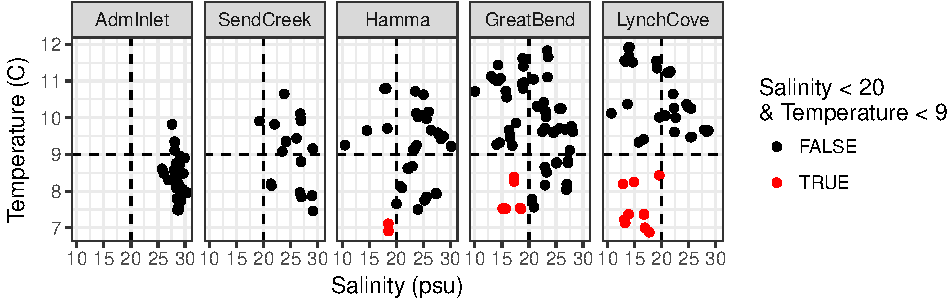
\includegraphics{20171117_Tides_and_eDNA_RPK_files/figure-latex/ContextualWaterData_WAEcology-1} 

}

\caption{\label{fig:SupplementalWaterChem}Contextual water data for the month of March from the Washington State Department of Ecology (https://fortress.wa.gov/ecy/eap/marinewq/mwdataset.asp). Plots are arranged north to south, with the southernmost point being Lynch Cove, near our sampled site of Twanoh. Red points indicate Temperature/Salinity data in the range of those in which we observed eDNA Community 2; these are far more common in the southern end of Hood Canal than in the north, which has a stronger oceanic influence. The data show more southern points in the Hood Canal have an increased likelihood of cold, fresh water in March (red points). These make up the following proportions: Admiralty Inlet = 0, Send Creek = 0, Hamma Hamma =0.05, Great Bend = 0.11, Lynch Cove = 0.28.}\label{fig:ContextualWaterData_WAEcology}
\end{figure}

\begin{table}

\caption{\label{tab:SupplTable_EcologySampling}Coordinates for WA Department of Ecology water quality sampling sites, which encompass the waters we sampled for the study presented in the main text.}
\centering
\begin{tabular}[t]{c|c|c}
\hline
Site Name & Latitude & Longitude\\
\hline
Admiralty Inlet & 48.03 & -122.6167\\
\hline
Send Creek & 47.667 & -122.82\\
\hline
Hamma Hamma & 47.5383 & -123.0083\\
\hline
Great Bend & 47.3567 & -123.0233\\
\hline
Lynch Cove & 47.3983 & -122.9283\\
\hline
\end{tabular}
\end{table}

\newpage

\section*{References}\label{references}
\addcontentsline{toc}{section}{References}

\hypertarget{refs}{}
\hypertarget{ref-Babson2006}{}
Babson AL., Kawase M., MacCready P. 2006. Seasonal and interannual
variability in the circulation of puget sound, washington: A box model
study. \emph{Atmosphere-Ocean} 44:29--45. DOI:
\href{https://doi.org/10.3137/ao.440103}{10.3137/ao.440103}.

\hypertarget{ref-camacho2009blast}{}
Camacho C., Coulouris G., Avagyan V., Ma N., Papadopoulos J., Bealer K.,
Madden TL. 2009. BLAST+: Architecture and applications. \emph{BMC
Bioinformatics} 10:421.

\hypertarget{ref-deiner2017environmental}{}
Deiner K., Bik HM., Mächler E., Seymour M., Lacoursière-Roussel A.,
Altermatt F., Creer S., Bista I., Lodge DM., Vere N de., others. 2017.
Environmental DNA metabarcoding: Transforming how we survey animal and
plant communities. \emph{Molecular Ecology}.

\hypertarget{ref-deiner_transport_2014-1}{}
Deiner K., Altermatt F. 2014. Transport Distance of Invertebrate
Environmental DNA in a Natural River. \emph{PLoS One} 9:e88786. DOI:
\href{https://doi.org/10.1371/journal.pone.0088786}{10.1371/journal.pone.0088786}.

\hypertarget{ref-helmuth2006living}{}
Helmuth B., Mieszkowska N., Moore P., Hawkins SJ. 2006. Living on the
edge of two changing worlds: Forecasting the responses of rocky
intertidal ecosystems to climate change. \emph{Annu. Rev. Ecol. Evol.
Syst.} 37:373--404.

\hypertarget{ref-huson2016megan}{}
Huson DH., Beier S., Flade I., Górska A., El-Hadidi M., Mitra S.,
Ruscheweyh H-J., Tappu R. 2016. MEGAN community edition-interactive
exploration and analysis of large-scale microbiome sequencing data.
\emph{PLoS Computational Biology} 12:e1004957.

\hypertarget{ref-jane2015distance}{}
Jane SF., Wilcox TM., McKelvey KS., Young MK., Schwartz MK., Lowe WH.,
Letcher BH., Whiteley AR. 2015. Distance, flow and PCR inhibition: EDNA
dynamics in two headwater streams. \emph{Molecular Ecology Resources}
15:216--227.

\hypertarget{ref-jerde2016influence}{}
Jerde CL., Olds BP., Shogren AJ., Andruszkiewicz EA., Mahon AR., Bolster
D., Tank JL. 2016. Influence of stream bottom substrate on retention and
transport of vertebrate environmental DNA. \emph{Environmental Science
\& Technology} 50:8770--8779.

\hypertarget{ref-kelly2016genetic}{}
Kelly RP., O'Donnell JL., Lowell NC., Shelton AO., Samhouri JF.,
Hennessey SM., Feist BE., Williams GD. 2016. Genetic signatures of
ecological diversity along an urbanization gradient. \emph{PeerJ}
4:e2444.

\hypertarget{ref-kelly2017multilocus}{}
Kelly RP., Closek CJ., O'Donnell JL., Kralj JE., Shelton AO., Samhouri
JF. 2017. Genetic and manual survey methods yield different and
complementary views of an ecosystem. \emph{Frontiers in Marine Science}
3:283. DOI:
\href{https://doi.org/10.3389/fmars.2016.00283}{10.3389/fmars.2016.00283}.

\hypertarget{ref-lahoz2015statistical}{}
Lahoz-Monfort JJ., Guillera-Arroita G., Tingley R. 2015. Statistical
approaches to account for false positive errors in environmental DNA
samples. \emph{Molecular Ecology Resources}.

\hypertarget{ref-leray_new_2013}{}
Leray M., Yang JY., Meyer CP., Mills SC., Agudelo N., Ranwez V., Boehm
JT., Machida RJ. 2013. A new versatile primer set targeting a short
fragment of the mitochondrial COI region for metabarcoding metazoan
diversity: Application for characterizing coral reef fish gut contents.
\emph{Frontiers in Zoology} 10:34.

\hypertarget{ref-mahe2015swarm}{}
Mahé F., Rognes T., Quince C., Vargas C de., Dunthorn M. 2015. Swarm v2:
Highly-scalable and high-resolution amplicon clustering. \emph{PeerJ}
3:e1420.

\hypertarget{ref-martin2011cutadapt}{}
Martin M. 2011. Cutadapt removes adapter sequences from high-throughput
sequencing reads. \emph{EMBnet.journal} 17:pp--10.

\hypertarget{ref-vegan}{}
Oksanen J., Blanchet FG., Kindt R., Legendre P., Minchin PR., O'Hara
RB., Simpson GL., Solymos P., Stevens MHH., Wagner H. 2015. \emph{Vegan:
Community ecology package}.

\hypertarget{ref-banzai}{}
O'Donnell JL. 2015. Banzai. \emph{GitHub repository}.

\hypertarget{ref-o2016indexed}{}
O'Donnell JL., Kelly RP., Lowell NC., Port JA. 2016. Indexed PCR primers
induce template-specific bias in large-scale DNA sequencing studies.
\emph{PloS one} 11:e0148698.

\hypertarget{ref-o2017spatial}{}
O'Donnell JL., Kelly RP., Shelton AO., Samhouri JF., Lowell NC.,
Williams GD. 2017. Spatial distribution of environmental DNA in a
nearshore marine habitat. \emph{PeerJ} 5:e3044.

\hypertarget{ref-MEC:MEC13481}{}
Port JA., O'Donnell JL., Romero-Maraccini OC., Leary PR., Litvin SY.,
Nickols KJ., Yamahara KM., Kelly RP. 2016. Assessing vertebrate
biodiversity in a kelp forest ecosystem using environmental DNA.
\emph{Molecular Ecology} 25:527--541. DOI:
\href{https://doi.org/10.1111/mec.13481}{10.1111/mec.13481}.

\hypertarget{ref-RcoreTeam}{}
R Core Team. 2016. \emph{R: A language and environment for statistical
computing}. Vienna, Austria: R Foundation for Statistical Computing.

\hypertarget{ref-renshaw2015room}{}
Renshaw MA., Olds BP., Jerde CL., McVeigh MM., Lodge DM. 2015. The room
temperature preservation of filtered environmental DNA samples and
assimilation into a phenol--chloroform--isoamyl alcohol DNA extraction.
\emph{Molecular Ecology Resources} 15:168--176.

\hypertarget{ref-royle2006generalized}{}
Royle JA., Link WA. 2006. Generalized site occupancy models allowing for
false positive and false negative errors. \emph{Ecology} 87:835--841.

\hypertarget{ref-sassoubre2016quantification}{}
Sassoubre LM., Yamahara KM., Gardner LD., Block BA., Boehm AB. 2016.
Quantification of environmental DNA (eDNA) shedding and decay rates for
three marine fish. \emph{Environmental Science \& Technology}
50:10456--10464.

\hypertarget{ref-schnell2015tag}{}
Schnell IB., Bohmann K., Gilbert MTP. 2015. Tag jumps
illuminated--reducing sequence-to-sample misidentifications in
metabarcoding studies. \emph{Molecular Ecology Resources} 15:1289--1303.

\hypertarget{ref-sigsgaard2016population}{}
Sigsgaard EE., Nielsen IB., Bach SS., Lorenzen ED., Robinson DP.,
Knudsen SW., Pedersen MW., Al Jaidah M., Orlando L., Willerslev E.,
others. 2016. Population characteristics of a large whale shark
aggregation inferred from seawater environmental DNA. \emph{Nature
Ecology \& Evolution} 1:0004.

\hypertarget{ref-spear2015using}{}
Spear SF., Groves JD., Williams LA., Waits LP. 2015. Using environmental
DNA methods to improve detectability in a hellbender
(\emph{cryptobranchus alleganiensis}) monitoring program.
\emph{Biological Conservation} 183:38--45.

\hypertarget{ref-taberlet2012environmental}{}
Taberlet P., Coissac E., Hajibabaei M., Rieseberg LH. 2012.
Environmental DNA. \emph{Molecular Ecology} 21:1789--1793.

\hypertarget{ref-thomsen_detection_2012}{}
Thomsen PF., Kielgast J., Iversen LL., Møller PR., Rasmussen M.,
Willerslev E. 2012. Detection of a diverse marine fish fauna using
environmental DNA from seawater samples. \emph{PloS One} 7:e41732.

\hypertarget{ref-thomsen2015environmental}{}
Thomsen PF., Willerslev E. 2015. Environmental DNA--An emerging tool in
conservation for monitoring past and present biodiversity.
\emph{Biological Conservation} 183:4--18.

\hypertarget{ref-MASS}{}
Venables WN., Ripley BD. 2002. \emph{Modern applied statistics with s}.
New York: Springer.

\hypertarget{ref-ggplot}{}
Wickham H. 2009. \emph{Ggplot2: Elegant graphics for data analysis}.
Springer-Verlag New York.

\hypertarget{ref-wilcox2016understanding}{}
Wilcox TM., McKelvey KS., Young MK., Sepulveda AJ., Shepard BB., Jane
SF., Whiteley AR., Lowe WH., Schwartz MK. 2016. Understanding
environmental DNA detection probabilities: A case study using a
stream-dwelling char salvelinus fontinalis. \emph{Biological
Conservation} 194:209--216.

\hypertarget{ref-treemapify}{}
Wilkins D. \emph{Treemapify: Draw treemaps in 'ggplot2'}.

\hypertarget{ref-yamamoto2016environmental}{}
Yamamoto S., Minami K., Fukaya K., Takahashi K., Sawada H., Murakami H.,
Tsuji S., Hashizume H., Kubonaga S., Horiuchi T., others. 2016.
Environmental DNA as a `snapshot'of fish distribution: A case study of
japanese jack mackerel in maizuru bay, sea of japan. \emph{PloS one}
11:e0149786.

\hypertarget{ref-zhang2014pear}{}
Zhang J., Kobert K., Flouri T., Stamatakis A. 2014. PEAR: A fast and
accurate illumina paired-end reAd mergeR. \emph{Bioinformatics}
30:614--620.

\end{document}